\cotefile{157-4}
\scanpage{98}
\mspage{91}
% archive sheet number: 97
Soit
\[
C=\deleted{\unsure{\mathrm{Filt}|A|F}}\underline{M}^{\pi}/\unsure{x|\chi}
\]
la catégorie suivante, les objets sont les triples
\[
(Z,i,\unsure{\alpha|u})\mid Z\in M^{\pi},\quad i\in I,\quad \alpha:Z\longrightarrow X_i,
\]
les flèches
\[
(Z,i,\alpha)\longrightarrow \overset{\unsure{{-}\,\smile|r\,u}}{(Z',i',\alpha')}
\]
sont les couples $(u,\lambda)$ \unsure{avec|où}
\[
u:Z\longrightarrow Z',\qquad \lambda:i\longrightarrow i'
\]
(i.e. on a $i\leq i'$, et $\lambda$ est l'unique flèche de $i$ dans $i'$)
tels que le diagramme
\diagram{\begin{tikzcd}[ampersand replacement=\&]
Z \arrow[r,"\alpha"] \arrow[d,"u"'] \& X_i \arrow[d,"{\text{transition }\unsure{\lambda x_{i',i}|\lambda^{i'}_{,i}|\lambda_{i',i}}}"] \\
Z' \arrow[r,"\alpha'"] \& X_{i'}
\end{tikzcd}}
commute. On peut donc définir $C$ comme le produit fibré dans le carré cartésien
\diagram{\begin{tikzcd}[ampersand replacement=\&]
\& C \arrow[r,"\text{cofibré}"] \arrow[d] \arrow[dl,dashed,"{\unsure{\mathscr F|\mathscr G|\xi}}"'] \& I \arrow[d,"{x:\unsure{X|i}\longmapsto X_i}"] \\
\underline M^{\pi} \& \underline M^{\pi}/E \arrow[l,dashed,"\text{source}"] \arrow[r,"\text{but}","\text{cofibré}"'] \& E
\end{tikzcd}}
\deleted{\unsure{Comme}} La fibre de $C$ en $i\in\deleted{\unsure{J|E}}I$ est $\mathrm{Filt}^{\pi}/X_i$. On a \deleted{\unsure{prouvé}}
% slanted; the curved leader attaches the lower addition at cancelled prouvé
\inserted{Comme b) $\Rightarrow$ \deleted{\unsure{a petite partie|la petite partie}} \unsure{première moitié de a)|première moitié de b)}). que} ($\underline M^{\pi}$ \unsure{est un|est une}

\scanpage{99}
\mspage{92}
% archive sheet number: 98
\unsure{syst..|syst.} de générateurs stricts de $\deleted{\unsure{E|F}}\underline M$, et
\inserted{$X_i\in\operatorname{Ob}\underline M$ \unsure{pour tt i|pour tt}.}
\[
X_i=\unsure{\underline{\lim}|\varinjlim}_{Z\in\underline M^{\pi}/X_i}Z
=\varinjlim_{\unsure{\partial|Z|\alpha|J}\,\unsure{\in|\deleted{I}|\deleted{J}}C_i}\unsure{\mathscr F|\mathscr G|\xi}|C_i,
\]
donc le système inductif donné \inserted{$(X_i)_{i\in I}$} sur $I$, à valeurs dans $X$, se déduit du syst. inductif (non \unsure{ordonné} en général) sur $C$, à valeurs dans $\underline M^{\pi}$, en ``intégrant'' sur les fibres de $C\longrightarrow I$.

D'ailleurs, comme $\underline M^{\pi}/E\unsure{\relbar|\longrightarrow}E$ est cofibré, \unsure{donc|et} propre, il en est de $=$ $C\longrightarrow I$, donc \deleted{\unsure{de former}} les $\varinjlim$ de $F$ sur les fibres $C_i$ \inserted{$(=\underline M^{\pi}/X_i)$} \inserted{forment} un foncteur covariant $I\longrightarrow E$, dont la limite inductive est celle de $F$.
% margin note written sideways
\margin{\uline{NB} Si on admet la validité de a), alors il en résulte \unsure{déjà} \unsure{ici}, que $\varinjlim_{i\in I}X_i\simeq\lim_{\alpha\in C}Z_\alpha$ est $\in M$. (Stabilité de $M$ \unsure{aux|par} \unsure{$\varinjlim$ grandes} devant $\pi$.)}

\deleted{Considérons tous \deleted{\unsure{les objets}} les \inserted{sous-catégories} \deleted{pleines} $C'_\alpha$ de $C$ \inserted{\uline{filtrantes $C_\alpha$}} de cardinal (tt l'ens des flèches) $\leq\pi$. \deleted{\unsure{car}} J'admets (cf plus bas) que \uline{$C^{\alpha}$ \unsure{lui-m.} est filtrant} (ce qui est \unsure{facile}: \unsure{il est même} \unsure{un objet|une catégorie} \unsure{conséquence} de \unsure{son être} filtrant), de sorte que $C$ est réunion des}
% slanted
\margin{\uline{C'est \unsure{faux}!!} \unsure{même pour} \unsure{un ensemble}, \unsure{supp.} \unsure{Mais} \unsure{si} $C$ \unsure{est un} \unsure{ensemble} \unsure{les objets de} $\mathrm{Filt}^{\pi}$ \unsure{sont $\pi$-accessibles} \unsure{pour} \unsure{les} \unsure{limites} $\ldots$}

\scanpage{100}
\mspage{93}
% archive sheet number: 99
Soit, pour tout $i\in I$, $\widetilde C_i$ l'ens ordonné
\[
\widetilde C_i=\{\text{sous-catégories }C'_i\text{ de }C_i=\underline M^{\pi}/X_i\mid
\begin{aligned}
&\operatorname{card}\operatorname{Fl}(C'_i)\leq\pi,\\
&C'_i\text{ filtrante}
\end{aligned}\}.
\]
J'admets pour l'instant le

\uline{Lemme} Pour \deleted{\unsure{tout}} tout, $X\in\deleted{\unsure{E|M^{\pi}}}\inserted{M^{\deleted{\unsure{\pi|\ast}}}}$, la catégorie $\deleted{\unsure{\underline M^{\pi}/X|C_i}}\inserted{\underline M^{\pi}/X}$ est filtrante.
\inserted{(\unsure{Bien|Par} l'hypothèse (b), \unsure{en ce que|on a que|en que} \unsure{tt élém de|tt pt de|tt partie de|tt objet de} $M$ est de la forme \unsure{dite dans a)|dit dans a)|et de dans}) \unsure{comme} $X_i\in M^{\deleted{\unsure{\pi|\ast}}}$, \unsure{par|puis} $C_i$ est filtrant,}
% margin note written sideways
\margin{Utiliser l'hypothèse \deleted{\unsure{précisée|forte}} que les éléments de $\mathrm{Filt}^{\pi}$ sont \unsure{$\pi$-accessibles|$\pi$-accessible}.}

Il en résulte, \deleted{\unsure{donc}} la réunion des $C'_i$ \inserted{$\in\widetilde C_i$} est $C_i$; et l'ensemble ordonné $\widetilde C_i$ est filtrant, \inserted{et} toute partie \inserted{$(C'_{i,\alpha})_{\alpha\in A}$ filtrante et} de cardinal $\leq\pi$ de $\unsure{\widetilde C'_i|\widetilde C_i}$ admet une borne supérieure $C'_{iA}$, savoir la réunion des $C'_{i\alpha}$. $\widetilde C_i$ est donc un ens ordonné $\pi$-adapté. \unsure{On}

On peut considérer les ens. ordonnés $\widetilde C_i$, pour $i\in I$ variable, comme les fibres d'une application croissante d'ens ordonnés
\[
p:\widetilde C\longrightarrow C,
\]
en \deleted{disant} \unsure{écrivant}
\[
\left\{\begin{aligned}
&(C'_i\subset C_i)\leq(C'_j\subset C_j)\\
&\text{ssi }i\leq j,\text{ et le foncteur canonique}\\
&\text{de transition }C_i\longrightarrow C_j\text{ applique }C'_i\\
&\text{dans }C'_j.
\end{aligned}\right.
\]
On voit donc que $\widetilde C$ est lui aussi filtrant et grand devant $\pi$.

\scanpage{101}
\mspage{94}
% archive sheet number: 100
\deleted{Il est \unsure{évident} que}
On définit un système inductif sur $\widetilde C$, à valeurs dans $\underline{\mathrm{Filt}}^{\pi}$, en posant
\[
Z_{\deleted{\unsure{\alpha}}C'_i}=\varinjlim_{\alpha\in C'_i(\unsure{\in|\subset}C_i\unsure{\neq|)=|=}\underline M^{\pi}/X_i)}Z_\alpha
\]
(\unsure{où|car} un $\alpha\in C_i$ est donné, je le rappelle, par
\[
Z_\alpha\xrightarrow{u_\alpha}X_i,\quad\text{avec }Z_\alpha\in M^{\pi}\subset\underline{\mathrm{Filt}}^{\pi}).
\]
Les $Z_{C'_i}$ ne sont plus forcément dans $M^{\pi}$, mais seulement dans $\mathrm{Filt}^{\pi}$. \deleted{\unsure{elles-mêmes}}

\deleted{(Alors à quoi ça \unsure{sert|servirait|servait} de \deleted{\unsure{avoir|voire}} \inserted{définir} \deleted{prendre} les $C_i$ \unsure{ci-dessus} comme $\underline M^{\pi}/X_i$, au lieu de $\underline{\mathrm{Filt}}^{\pi}/X_i$?)}

Le système inductif
\[
(Z_{C'_i})_{C'_i\in\widetilde C_i}
\]
est \deleted{\unsure{bien}} \inserted{\unsure{parfaitement}} adapté à la filtration \unsure{cardinale|cardinal} par le cardinal $\pi$, et il est immédiat que sa $\varinjlim$ est \inserted{donc}
\[
\varinjlim_{\alpha\in\operatorname{Ob}C_i=\underline M^{\deleted{\unsure{\ast|\pi}}\pi}/X_i}Z_\alpha=X_i\unsure{\in|\in_{\varphi}}M.
\]
Donc par b), l'ens \deleted{\unsure{des $C'_i$}} $\widetilde C_M$ des $C'_i\deleted{\unsure{\ast}}\in\widetilde C_i$ tels que $Z_{C'_i}\in M$ (donc $Z_{C'_i}\in M^{\pi}$) est cofinal dans $\unsure{\widetilde C_i|\widetilde C}$, Il s'ensuit donc que l'ens. $\widetilde C_M$ est lui-aussi cofinal dans $\widetilde C$.

\scanpage{102}
\mspage{95}
% archive sheet number: 101
On vérifie aussi immédiatement que
\[
\varinjlim_{\alpha\in\widetilde C}Z_\alpha=\unsure{\underline{\lim}|\varinjlim}X_i=X
\]
donc, $\widetilde C_M$ étant cofinal,
\[
\underline{\lim}_{\alpha\in\widetilde C_M}Z_\alpha=X.
\]
\deleted{Il reste \unsure{bien} \unsure{entendu} que le syst. inductif $Z_\alpha$ sur $\widetilde C$ \unsure{tout entier}, \unsure{restreint|induit} sur $\widetilde C_M$,}

Au total, on est arrivé à représenter $X$ sous la forme
\[
X=\varinjlim_{\alpha\in A}X_\alpha
\]
cette fois les $X_\alpha$ sont \uline{dans $M^{\pi}$} (pas seulement dans $M$), et $A$ est \deleted{\unsure{donc}} \inserted{grand devant $\pi$}. \deleted{adapté à $\pi$ (pas seulement grand devant $\pi$)} Mais on ne sait pas que \deleted{les} toute partie \inserted{filtrante $B$} de cardinal $\leq\pi$ de $A$ admet une borne sup \inserted{$\alpha_B$} dans $A$, et encore moins que $X_{\alpha_B}=\underline{\lim}_{\alpha\in B}X_\alpha$. Donc on ne peut \inserted{encore} appliquer directement b). S'il ne s'agissait que de prouver \inserted{\unsure{la deuxième moitié de|la première moitié de}} a), \unsure{où|ou} on suppose déjà les $X_i\in M^{\pi}$ et $I$ grand devant $I$, on n'a rien gagné du tout par \unsure{nos} \unsure{labeurs}!
% slanted
\margin{Si on \unsure{supprime|suppose} ($\unsure{a_\pi|a^\pi|a}$) cet argument \unsure{nous} prouve \unsure{alors} que $M$ est stable par $\varinjlim$ grandes devant $\pi$.}

\scanpage{103}
\mspage{96}
% archive sheet number: 102
Mais revenons à ce cas
\[
X=\varinjlim X_i\quad\left|\begin{aligned}
&X_i\in M^{\pi}\\
&I\text{ grand devant }\pi
\end{aligned}\right.,
\]
et \unsure{introduisons} à nouveau
\[
\widetilde I=\{I'\subset I\mid I'\text{ filtrant, de cardinal }\leq\pi\},
\]
donc cette fois $\widetilde I$ est \deleted{\unsure{fort}} bien adapté à $\pi$ (filtrant, et toute partie \inserted{filtrante} de cardinal $\leq\pi$ a une borne supérieure), et si on pose
\[
X_{\widetilde i}=\varinjlim_{i\in\unsure{I'_{\widetilde i}|J'_{\widetilde i}}}X_i,
\]
on voit que ce syst. inductif
\[
(X_{\widetilde i})_{\widetilde i\in\widetilde I}
\]
est parfaitement adapté à $\pi$ \unsure{et|à} la filtr. cardinale. De plus, \deleted{\unsure{par une|pour une} application canonique
\[
I\longrightarrow\widetilde I\qquad i\longmapsto\{i\},
\]
(pas \unsure{croissant|croissante}, \unsure{qu'il est évident}), et $I$ est}
je dis que l'ens $\widetilde I_M$ est \uline{cofinal} dans $\widetilde I$. En effet,
\deleted{soit $I'\in\widetilde I$, et soit $i_0$ un majorant de $I'\deleted{\unsure{\subset|\in}}I$ dans $I$. Soit}
$\widetilde I_M$ contient le sous-ensemble $\widetilde I_0$ \unsure{formé|formée|fermé|fermée} des $I'\in\widetilde I$ qui ont un \deleted{plus} grand élément -- et $\widetilde I_0$ est bien cofinal! Maintenant, on peut appliquer,

\scanpage{104}
\mspage{97}
% archive sheet number: 103
le \unsure{``il suffit''|'il suffit'} dans b), qui \deleted{prouve} \inserted{assure} que $X=\unsure{\underline{\lim}|\varinjlim}X_i\in M$, qed.

\uline{NB} On a prouvé $b\Rightarrow a$, sans utiliser \unsure{l'hyp. faite|l'hyp.thèse|l'hypothèse} que tt objet de $\mathrm{Filt}^{\pi}$ est $\pi$-accessible. Mais on a utilisé cette hypothèse pour prouver que b \deleted{implique} (ou a) implique que $M$ est stable par $\underline{\lim}$ grandes devant $\pi$ (lemme 2, p. 90).

$a\overset{?}{\Longrightarrow}b$. Le ``il suffit'' de b) est conséquence immédiate de a). Je veux prouver que si, dans \deleted{le \unsure{même système}} \inserted{système \inserted{inductif}} \deleted{\unsure{parf.}} \inserted{$\pi$-adapté} $(X_i)_{i\in I}$ de limite $X$, on a $X\in M$, alors $I_M$ est cofinal dans $I$. Mais par hyp. a), on a encore
\[
\deleted{\unsure{A|M}}X=\varinjlim_JY_j,
\]
avec $J$ grand devant $\pi$, les $Y_j$ dans $M^{\pi}$. \deleted{Soit $i\in I$}, Admettons que $\mathrm{Filt}^{\pi}\subset E_\pi$ i.e tt élément de $\mathrm{Filt}^{\pi}$, en particulier les $X_i$, sont \deleted{bien} $\pi$-accessibles.

Je pense que je n'arriverai pas à prouver $a_\pi\Rightarrow b_\pi$, mais seulement ceci: Si $\pi'$ est un cardinal $>\pi$ (disons le successeur de $\pi$ \unsure{pris|$\xi$} dans l'\deleted{\unsure{ens}} \inserted{suite ordinale} des cardinaux) alors
\[
a_\pi\Longrightarrow b_{\pi'}.
\]
\deleted{Donc dans les arguments qui précèdent, on supposera $I$ grand devant $\pi'$, non seulement grand devant $\pi$. Soit \inserted{donc} $\alpha_0$ le plus petit ordinal qui soit grand devant $\pi$, il est de cardinal $\leq\pi'$ (car lorsque $\pi'>\pi$, le plus petit ordinal $\unsure{\alpha'_0|\alpha'}$ de cardinal $\pi'$ est grand dev. \unsure{à} $\pi$ car $\pi<\pi'$, \unsure{donc} $\alpha'\geq\alpha'_0$, donc $\pi'\unsure{\leq|=}\operatorname{card}\alpha'\geq\operatorname{card}\unsure{\alpha_0|\pi_0}$.}

\scanpage{105}
\mspage{98}
% archive sheet number: 104
\deleted{On \unsure{a|va} construire \deleted{deux} \inserted{des} systèmes inductifs \inserted{de $(X_i)$, $(Y_j)$} indexés par les ordinaux $\alpha<\alpha_0$, en procédant par récurrence transfinie.}
Ceci va résulter du

\uline{Lemme} 3 Soient $X=\varinjlim_I X_i$, $X\simeq\unsure{\underline{\lim}|\varinjlim}_JY_j$ deux représentations de $X$ sous forme de $\underline{\lim}$ filtrantes, avec $I$ grand devant $\pi'$, $J$ grand devant $\pi$, avec $\pi,\pi'$ deux cardinaux tels que $\pi'>\pi$. On suppose $(X_i)_{i\in I}$ $\pi'$-adapté, i.e pour toute partie filtrante $I'$ de $I$ de cardinal $\leq\pi'$, $I'$ a une borne supérieure $i_{I'}$ et $X_{i_{I'}}=\varinjlim_{i\in I'}X_i$.

Alors pour \unsure{tout|tt} $i\in\unsure{I|\Delta}$, on peut trouver une partie $I'$ de $I$, \inserted{contenant $i$,} \uline{\unsure{grande|grand} devant $\pi$}, de cardinal $\leq\pi'$, \deleted{bien ordonnée} et une partie $J'$ de $J$, \deleted{\unsure{cofinale|cofinalement}} \inserted{\unsure{quelqs|quelques|quelque}} \deleted{application} un isomorphisme
\[
I'\xrightarrow{\unsure{\lambda|\simeq|\sim}}J'
\]
et une application \inserted{\unsure{str.|stri.}} \unsure{croissante|croissant} $\unsure{\mu|u}:J'\longrightarrow I'$, \deleted{tels que} et des homs

\scanpage{106}
% archive sheet number: 105
% printed form: ruled stationery without printed words
$\overline{\underline{\mathrm{XIV}}}$

Carrés h-cartésiens et \unsure{ho-cocartésiens|h-cocartésiens}

\scanpage{108}
\mspage{\textcircled{1}}
% archive sheet number: 107 (upper left)
\diagram{\begin{tikzcd}[ampersand replacement=\&,column sep=small,execute at end picture={\draw ([xshift=-.4em,yshift=.8em]\tikzcdmatrixname-1-1.north west) rectangle ([xshift=.4em,yshift=-.3em]\tikzcdmatrixname-1-2.south east);}]
A \arrow[r,"i"] \& B \arrow[r,"j"] \arrow[d,bend right=15] \& C \arrow[r,"d"] \arrow[d,equal] \& \Sigma^1 A \arrow[r,"\Sigma(i)"] \& \Sigma B \arrow[r,"\Sigma(j)"] \& \Sigma C \arrow[r,"\Sigma(d)"] \& \Sigma^2 A \arrow[r] \& \unsure{\sim|\cdots} \\
\& \unsure{\varphi|\phi} \& C(i)
\end{tikzcd}}

\diagram{\begin{tikzcd}[ampersand replacement=\&,column sep=small,execute at end picture={\draw ([xshift=-.4em,yshift=.8em]\tikzcdmatrixname-1-1.north west) rectangle ([xshift=.4em,yshift=-.3em]\tikzcdmatrixname-1-2.south east);}]
X \& Y \arrow[l,"p"'] \& Z \arrow[l,"q"'] \& \Omega X \arrow[l,"\partial"'] \& \Omega Y \arrow[l,"\Omega(p)"'] \& \unsure{\Omega(Z)|\Omega Z} \arrow[l,"\Omega(q)"'] \& \Omega^2 X \arrow[l,"\Omega(\partial)"'] \\
\& \unsure{\rho|e} \arrow[u,bend right=15]
\end{tikzcd}}

% Main array; empty cells are the unlabelled continuation vertices on the sheet.
\diagram{\begin{tikzcd}[ampersand replacement=\&,column sep=.4em,row sep=1.2em,execute at end picture={\draw ([xshift=-1.1em,yshift=-.6em]\tikzcdmatrixname-3-5.south) .. controls ([xshift=-.35em,yshift=-.65em]\tikzcdmatrixname-3-5.south) and ([xshift=-.2em,yshift=-.3em]\tikzcdmatrixname-3-5.south) .. ([xshift=.8em,yshift=-.4em]\tikzcdmatrixname-3-5.south);}]
{} \& \vdots \& \vdots \& \vdots \& \vdots \& {} \& {} \& {} \& {} \\
{} \& \pi_{\unsure{2|1}}(A,X) \arrow[l] \arrow[d] \& \pi_2(A,Y) \arrow[l] \arrow[d] \& \pi_2(\unsure{A|B},Z) \arrow[l] \arrow[d] \& {} \arrow[l] \arrow[d] \& {} \& {} \& {} \& {} \\
{} \& \pi_1(C,X) \arrow[l] \arrow[d,leftrightarrow] \& \pi_1(C,Y) \arrow[l,two heads] \arrow[d] \& \pi_1(C,Z) \arrow[l] \arrow[d] \& \unsure{\infty|0} \arrow[l] \arrow[d] \& {} \& {} \& {} \& {} \\
{} \& \pi_1(B,X) \arrow[l] \arrow[d] \& \pi_1(B,Y) \arrow[l] \arrow[d] \& \pi_1(B,Z) \arrow[l] \arrow[d] \& {} \arrow[l] \arrow[d] \& {} \& {} \& {} \& {} \\
{} \& \pi_1(A,X) \arrow[l] \arrow[d] \& \pi_{\unsure{0|1}}(A,\unsure{Y|X}) \arrow[l] \arrow[d] \& \pi_0(A,Z) \arrow[l] \arrow[d] \& \pi_2(A,X) \arrow[l] \arrow[d] \& {} \arrow[d] \& {} \& {} \& {} \\
{} \& \unsure{\deleted{\pi_{-1}}\pi_0|\deleted{\pi_1}\pi_0|\pi_0}(C,X) \arrow[d] \& \pi_0(C,Y) \arrow[l] \arrow[d] \& \pi_0(C,Z) \arrow[l] \arrow[d] \& \pi_1(C,X) \arrow[l] \arrow[d] \& {} \arrow[l] \arrow[d] \& {} \& {} \& {} \\
{} \& \deleted{\pi_{-1}}\pi_0(B,X) \arrow[d] \& \pi_0(B,Y) \arrow[l] \arrow[d] \& \pi_0(B,Z) \arrow[l] \arrow[d] \& \pi_1(B,X) \arrow[l] \arrow[d] \& {} \arrow[l] \arrow[d] \& {} \& {} \& {} \\
{} \& |[draw,circle,inner sep=2pt]|{\deleted{\pi_{-1}}\pi_0(A,X)} \& \pi_0(A,Y) \arrow[l,two heads] \& \pi_0(A,Z) \arrow[l] \arrow[d] \& \pi_1(A,X) \arrow[l] \arrow[d] \& {} \arrow[l] \arrow[d] \& {} \& {} \& {} \\
{} \& {} \& {} \& {} \& \pi_0(C,X) \arrow[d] \& {} \arrow[l] \arrow[d] \& {} \& {} \& {} \\
{} \& {} \& {} \& {} \& \pi_0(B,X) \arrow[d] \& {} \arrow[l] \arrow[d] \& {} \& {} \& {} \\
{} \& {} \& {} \& {} \& \pi_0(A,X) \& \pi_0(A,Y) \arrow[l] \& \pi_0(A,Z) \arrow[l] \& \pi_1(A,X) \arrow[l] \arrow[d] \& {} \arrow[l] \arrow[d] \\
{} \& {} \& {} \& {} \& {} \& {} \& {} \& \pi_0(C,\unsure{\Lambda|X}) \arrow[d] \& {} \arrow[l] \arrow[d] \\
{} \& {} \& {} \& {} \& {} \& {} \& {} \& \pi_0(\unsure{D|B},X) \arrow[d] \& {} \arrow[l] \arrow[d,no head] \\
{} \& {} \& {} \& {} \& {} \& {} \& {} \& \unsure{\pi_0(A,X)|\pi_0(A,X} \& {}
\arrow[from=5-2,to=8-5,dashed,no head,shorten <=2em,shorten >=2em]
\end{tikzcd}}

NB\unsure{,|:|;}
\[
\pi_i(\Sigma^j\unsure{S|\mathscr S|\mathbb S},\Omega^{\unsure{k|h|m}}T)\simeq\pi_{i\unsure{+|\wedge}j+\unsure{m|k}}(S,T\unsure{)|),}
\]

\figure{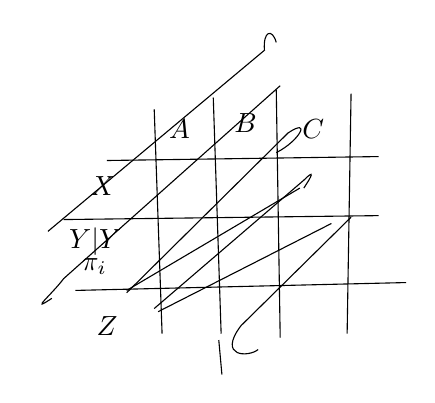
\begin{tikzpicture}[x=1cm,y=1cm]
\draw (.9,-.2)--(.8,2.65) (1.65,-.2)--(1.55,2.8) (2.4,-.25)--(2.35,2.9) (3.25,-.2)--(3.3,2.85);
\draw (.2,2)--(3.65,2.05) (-.35,1.25)--(3.65,1.3) (-.2,.35)--(4,.45);
\draw (-.55,1.1)--(2.2,3.4) .. controls (2.18,3.65) and (2.3,3.68) .. (2.35,3.5);
\draw (-.5,.25) .. controls (-.8,.05) and (-.5,.3) .. (-.35,.5) --(2.4,2.95);
\draw (.45,.32)--(2.5,2.35) .. controls (2.8,2.55) and (2.65,2.25) .. (2.35,2.1);
\draw (.8,.12)--(2.7,1.75) .. controls (2.85,1.9) and (2.8,1.8) .. (2.7,1.65);
\draw (1.9,-.1) .. controls (1.6,-.5) and (2,-.5) .. (2.12,-.4);
\draw (1.9,-.1)--(3.3,1.28);
\draw[thin] (.45,.35)--(2.65,1.65) (.85,.08)--(3.05,1.2);
\draw (1.62,-.28)--(1.66,-.72);
\node at (1.12,2.4) {$A$}; \node at (1.96,2.47) {$B$}; \node at (2.82,2.4) {$C$};
\node at (.15,1.67) {$X$}; \node at (.05,.97) {$\unsure{Y|\deleted{Y}}$};
\node at (.04,.65) {$\pi_i$}; \node at (.2,-.1) {$Z$};
\end{tikzpicture}}

\diagram{\begin{tikzcd}[ampersand replacement=\&,column sep=small,row sep=1.3em,execute at end picture={\draw ([xshift=-.5em]\tikzcdmatrixname-1-2.north west)--([xshift=-.5em]\tikzcdmatrixname-4-2.south west);\draw ([xshift=-.5em]\tikzcdmatrixname-1-3.north west)--([xshift=-.5em]\tikzcdmatrixname-4-3.south west);\draw ([xshift=-.5em]\tikzcdmatrixname-1-4.north west)--([xshift=-.5em]\tikzcdmatrixname-4-4.south west);\draw (\tikzcdmatrixname-1-5.north east)--(\tikzcdmatrixname-4-5.south east);\draw (\tikzcdmatrixname-2-1.north west)--(\tikzcdmatrixname-2-5.north east);}]
\& A \arrow[d] \& B \arrow[d] \& C \arrow[d] \& {} \\
X \& \pi_i(A,X) \arrow[d] \& \pi_i(B,X) \arrow[l,leftrightarrow] \arrow[d] \& \pi_i(C,X) \arrow[l] \arrow[d] \& {} \arrow[l,"d_X"] \\
Y \& \pi_i(A,Y) \arrow[d] \& \pi_i(B,Y) \arrow[l] \arrow[d,phantom,"\unsure{\uparrow|0|\circ|\downarrow}" description] \& \pi_i(C,Y) \arrow[l] \arrow[d] \& {} \arrow[l,"d_Y"] \\
Z \& \pi_i(A,Z) \arrow[d] \& \pi_i(B,Z) \arrow[l] \& \pi_i(C,Z) \arrow[l] \& {} \arrow[l,"d_Z"] \\
\& {}
\end{tikzcd}}

\scanpage{109}
\mspage{A 3}
% archive sheet number: 108
% Faint reversed diagram strokes in the upper margin are show-through.
ou moins grossières, plus ou moins subtiles, suivant l'intéressé. Je ne prétends nullement y faire exception. La lecture de mon témoignage ne laissera, j'espère, aucun doute à ce sujet.

Il est vrai aussi que l'ambition la plus dévorante est impuissante à découvrir le moindre énoncé mathématique, ou à le démontrer - tout comme elle est impuissante (par exemple) à ``faire bander'' (au sens propre du terme). Qu'on soit femme ou homme, ce qui ``fait bander'' n'est nullement l'ambition, le désir de briller, d'exhiber une puissance, sexuelle en l'occurence - bien au contraire ! Mais c'est la perception aigüë de quelque chose de fort, de très réel et de très délicat à la fois. On peut l'appeler ``la beauté'', et c'est là un des mille visages de cette chose-là. D'être ambitieux n'empêche pas forcément de sentir parfois la beauté d'un être, ou d'une chose, d'accord. Mais ce qui est sûr, c'est que ce n'est \mbox{p a s} l'ambition qui nous la fait sentir...

L'homme qui, le premier, a découvert et maîtrisé le feu, était quelqu'un exactement comme toi et moi. Pas du tout ce qu'on se figure sous le nom de ``héros'', de ``demi-dieu'' et j'en passe. Sûrement, comme toi et comme moi, il a connu la morsure de l'angoisse, et la pommade vaniteuse éprouvée, qui fait oublier la morsure. Mais au moment où il a ``connu'' le feu, il n'y avait ni peur, ni vanité. Telle est la vérité dans le mythe héroïque. Le mythe devient insipide, il devient pommade, quand il nous sert à nous cacher un \mbox{a u t r e} aspect des choses, tout aussi réel et tout aussi essentiel.

Mon propos dans Récoltes et Semailles a été de parler de l'un et de l'autre aspect - de la pulsion de connaissance, et de la peur et de ses antidotes vaniteux. Je crois ``comprendre'', ou du moins \mbox{c o n n a î t r e} la pulsion et sa nature. (Peut-être un jour découvrirai-je, émerveillé, à quel point je me faisais illusion ...) Mais pour ce qui est de la peur et de la vanité, et les insidieux blocages de la créativité qui en dérivent, je sais bien que je n'ai pas été au fond de cette grande énigme. Et j'ignore si je verrai jamais le fond de ce mystère, pendant les années qui me restent à vivre ...

En cours d'écriture de Récoltes et Semailles deux images ont émergé, pour représenter l'un et l'autre de ces deux aspects de l'aventure humaine. Ce sont \mbox{l ' e n f a n t} (alias \mbox{l' o u v r i e r}), et le \mbox{P a t r o n}. Dans la Promenade qu'on va faire tantôt, c'est de ``l'enfant'' qu'il sera question presque exclusivement. C'est lui aussi qui figure dans le sous-titre ``\mbox{L ' e n f a n t \quad e t \quad l a \quad M è r e}''. Ce nom va s'éclairer, j'espère, au cours de la promenade.

\scanpage{110}
\mspage{\textcircled{2}}
% archive sheet number: 109
\[
Z(\unsure{\delta|r})\longrightarrow Z(p_0)\times Z(p_1)
\]

\deleted{\diagram{\begin{tikzcd}[ampersand replacement=\&,column sep=small,row sep=small]
{} \& {} \& Z'_0 \arrow[d] \& \bullet \arrow[l] \\
{} \& {} \& \unsure{X_{01}|Z_{01}} \arrow[ddll,phantom] \arrow[ddl] \& \unsure{\overline{Z}'_1|\Sigma'_1} \arrow[l] \\
Z_0 \arrow[d] \& Z'_0 \arrow[l,"\sim"'] \arrow[d] \arrow[uur,no head] \& \unsure{e|\varepsilon} \arrow[l] \arrow[d,no head] \\
X_0 \arrow[d,no head] \& X_0\times_S X_1 \arrow[l] \arrow[d] \& Z'_1 \arrow[l] \arrow[d,"\unsure{2|?}"] \arrow[uur] \\
S \& X_1 \arrow[l] \& Z_1 \arrow[l]
\end{tikzcd}}}

\diagram{\begin{tikzcd}[ampersand replacement=\&,execute at end picture={\draw ([xshift=-1em,yshift=1.8em]\tikzcdmatrixname-1-1.north west)--([xshift=-1.4em,yshift=-1.8em]\tikzcdmatrixname-1-1.south west);}]
\unsure{Z|\lambda} \arrow[r] \& Z(\delta) \arrow[r] \& Z(p_0)\times Z(p_1)
\end{tikzcd}}

\diagram{\begin{tikzcd}[ampersand replacement=\&,column sep=small,row sep=small,execute at end picture={\draw ([yshift=.6em]\tikzcdmatrixname-2-1.north west)--([xshift=.8em,yshift=.6em]\tikzcdmatrixname-2-4.north east)--([xshift=.8em,yshift=-.3em]\tikzcdmatrixname-2-4.south east);\draw (\tikzcdmatrixname-3-2.south west)--(\tikzcdmatrixname-3-4.south east);}]
\& Z(\alpha) \arrow[d,"\sim"] \\
\Omega(Z(p_0)\times Z(p_1)) \arrow[r] \& X_{22} \arrow[r] \& Z(\delta) \arrow[r,"\alpha"] \& Z(p_0)\times Z(p_1) \\
{} \arrow[u,dotted] \& X_{22} \arrow[r] \& X_{12} \arrow[r] \arrow[u] \& \unsure{X_{02}|Z_{02}}=Z(p_1) \arrow[u]
\end{tikzcd}}

\diagram{\begin{tikzcd}[ampersand replacement=\&,column sep=small]
\deleted{\unsure{X_{11}|X_1}} \arrow[r,leftrightarrow] \& X_{\unsure{11|tt}} \arrow[r] \& X_{10}\times_{X_{00}}X_{01} \arrow[d] \\
X_{22} \arrow[ur] \arrow[r,leftrightarrow] \& e \arrow[ur] \arrow[r,phantom,"\overset{\unsure{\cdot|\bullet}}{\unsure{\leftrightarrow|\longrightarrow}}" description] \& \unsure{\dot X_{00}|X_{00}}
\end{tikzcd}}

\diagram{\begin{tikzcd}[ampersand replacement=\&,column sep=small,row sep=1.7em,execute at end picture={\node[anchor=east] at ($(\tikzcdmatrixname-1-1)!0.5!(\tikzcdmatrixname-4-1)+(-1,0)$) {$\left\{\rule{0pt}{10em}\right.$};\node[anchor=east] at ($(\tikzcdmatrixname-2-1)!0.5!(\tikzcdmatrixname-4-1)+(-.6,0)$) {$\left\{\rule{0pt}{7em}\right.$};\node[anchor=east] at ($(\tikzcdmatrixname-3-1)!0.5!(\tikzcdmatrixname-4-1)+(-.25,0)$) {$\left\{\rule{0pt}{3.5em}\right.$};}]
\Omega X_{00} \arrow[d] \& \Omega X_{01} \arrow[l] \arrow[d] \& \Omega(X_{02}) \arrow[l] \arrow[d] \& \Omega^2 X_{00} \arrow[l] \arrow[d] \arrow[dl,no head,decorate,decoration={snake,amplitude=.4mm,segment length=2mm}] \\
X_{20} \arrow[d] \& X_{21} \arrow[l,"r_1"'] \arrow[d] \& |[draw]|X_{22} \arrow[l] \arrow[d] \arrow[dl,decorate,decoration={snake,amplitude=.4mm,segment length=2mm},"e"'] \& \Omega(X_{20}) \arrow[l] \arrow[d] \\
\unsure{X_{00}|X_{10}} \arrow[d,"p_0"'] \& X_{11} \arrow[l,"\unsure{q_0|q_1}"'] \arrow[d,"q_0"] \arrow[dl,dashed,"\delta"'] \& X_{1,2} \arrow[l] \arrow[d,"r_0"] \& \Omega X_{10} \arrow[l] \arrow[d] \\
X_{00} \& X_{01} \arrow[l,"p_1"] \& X_{02} \arrow[l] \& \Omega X_{00} \arrow[l] \arrow[d] \\
\& \& \& X_{20} \arrow[d] \\
\& \& \& X_{10} \arrow[d] \\
\& \& \& X_{00}
\end{tikzcd}}

\fbox{\begin{tabular}{l}\unsure{diagramme} des\\18 fibres\end{tabular}}

(ou des 12 fibres?)

\unsure{Si}
\[
\left\{\begin{aligned}
&p_0,p_1\text{ et}\\
&X_{11}\xrightarrow{\pi}X_{10}\times_{X_{00}}X_{01}
\end{aligned}\right.
\]
\unsure{fibrations} \deleted{\unsure{s}}
\unsure{définissons} \deleted{$X_{20},X_{21},X_{0,2},X_{1,2}$}
$X_{02},X_{1,2},X_{20},X_{21}$ comme fibres des $p_1,q_1$, $p_0,q_0$, on trouve que $r_0,r_1$ \unsure{sont des fibrations}, et leurs fibres s'identifient à \unsure{la} fibre de \deleted{$\unsure{X_{22}\to|X_{11}\to}$} $\pi$, de façon \unsure{précise} \unsure{dans|ds}
\diagram{\begin{tikzcd}[ampersand replacement=\&]
X_{21} \arrow[d,"\alpha_1"'] \\
X_{11} \& X_{1,2} \arrow[l,"\alpha_0"']
\end{tikzcd}}
\deleted{\unsure{Les|les|Et}} $Z(r_1)\subset\deleted{\unsure{Z|X}}\unsure{X_{22}|X_{21}}$ et $Z(\unsure{r_2|r_0})\subset X_{1,2}$ \unsure{ont|sont} $=$ \unsure{image|images} \deleted{$\unsure{Z_{22}|X_{22}}$} dans $X_{11}$, et $\alpha_1$ et $\alpha_0$ \unsure{induisent} des \unsure{iso.}
\diagram{\begin{tikzcd}[ampersand replacement=\&]
Z(r_1) \arrow[r,"\sim"] \& X_{22} \& Z(r_0) \arrow[l,"\sim"']
\end{tikzcd}}.

\scanpage{111}
\mspage{422}
% archive sheet number: 110
% Dark reversed diagram strokes show through the reused typed sheet.
J'avais eu tant de mal à l'entendre, parce que mon esprit était resté frais et alerte, tout frétillant de continuer sur sa lancée, comme s'il avait une vie autonome, totalement séparée de celle du corps. Il était même si frais et si frétillant qu'il avait le plus grand mal à tenir compte du besoin de sommeil du corps, refusant mordicus de démordre des tâches auxquelles il était attelé, et repoussant constamment jusqu'aux limites de l'épuisement l'échéance du sommeil, cet empêcheur de tourner en rond !

Pendant toute ma vie et jusqu'à il y a trois ou quatre ans, la capacité illimitée de récupération par un sommeil profond et prolongé, avait été le pendant solide et salutaire à des investissements d'énergie parfois démesurés : quand le sommeil est sûr, on ne craint plus rien, on peut se permettre (sans que ce soit folie) de se lancer à corps perdu et jusqu'à épuisement dans des orgies de travail - quitte à se rattrapper par des orgies de sommeil réparateur ! Cette capacité qui toute ma vie m'avait semblé aller de soi tout autant que la capacité de travail, la capacité de découverte (et sûrement les deux sont intimement reliées...), a fini en ces dernières années par s'élimer, et parfois par disparaître, pour des raisons que je discerne mal à présent, et que je n'ai pas vraiment fait effort encore de sonder. De plus en plus, quand, après une longue journée passée sur ma \unsure{machine|mochine} à écrire (ou sur des notes manuscrites) et obéissant aux injonctions de mon corps qui refuse de continuer, je me résouds enfin à aller me coucher, la position allongée (et le soulagement partiel qu'elle fournit à la tension de la position assise) relance aussitôt la réflexion. Celle-ci repart de plus belle, pendant des heures voire pour la nuit entière (ou plutôt ce qui en reste...). J'ai beau me rendre compte que le système n'est pas rentable (à supposer même qu'il soit \mbox{v i v a b l e} à la longue), vu que (chez moi du moins) une réflexion prolongée sans le support de l'écriture finit par tourner en rond, par devenir souvent une sorte de remâchage - le mauvais pli est bien pris, et a tendance à s'empirer. Il était devenu, il me semble, \mbox{l e} grand foyer de dispersion d'énergie dans ma vie en ces dernières années, alors que d'autres mécanismes de dispersion se sont éliminés un à un, progressivement, au fil des ans.

Si ce mécanisme-là s'est enraciné dans ma vie avec une telle ténacité, si j'ai été disposé pendant toutes ces dernières années à payer un tel prix, c'est sûrement que quelque chose en moi y a trouvé son compte, et y retrouverait son compte le moment venu. Ce ne serait pas un luxe que j'examine la situation de près - et plus d'une fois au cours des quatre mois écoulés j'ai été sur le point de le faire.

\scanpage{112}
\mspage{\textcircled{3}}
% archive sheet number: 111
\diagram{\begin{tikzcd}[ampersand replacement=\&]
S \arrow[r,maps to] \& \unsure{\varnothing|\phi} \arrow[r] \& e \arrow[r,phantom,"\unsure{{-}|\to}"] \& T
\end{tikzcd}}

\deleted{$\operatorname{Hom}(S,T)$
\diagram{\begin{tikzcd}[ampersand replacement=\&]
\delta \arrow[r] \& p_1
\end{tikzcd}}}

\deleted{$Z(\delta)=Z(p_1)$}

\diagram{\begin{tikzcd}[ampersand replacement=\&]
X_{22}\simeq Z(\alpha) \arrow[r,"?"] \& X_{12}=Z(q_1)
\end{tikzcd}}

\diagram{\begin{tikzcd}[ampersand replacement=\&]
\alpha \arrow[r,"?"] \& q_1
\end{tikzcd}}

\diagram{\begin{tikzcd}[ampersand replacement=\&,row sep=small]
Z(\delta) \arrow[r,"\alpha"] \arrow[dd,bend right=10] \& \underbrace{Z(p_0)\times Z(p_1)}_{X_{20}\times X_{02}} \arrow[d] \\
\& X_{20} \arrow[d] \\
X_{11} \arrow[r] \& X_{10}
\end{tikzcd}}

\figure{\begin{tikzpicture}[x=.01cm,y=-.01cm,line cap=round]
\draw[line width=.5pt] (46,64)--(43,78); \fill (42,92) circle[radius=1.4pt];
\draw[line width=1pt] (211,84)--(208,104)--(212,112);
\draw[line width=.8pt] (169,219)--(167,236); \draw (164,251)--(168,254)--(176,246);
\fill (295,188) circle[radius=1.2pt];
\draw[line width=1.1pt] (344,372)--(353,369);
\draw[line width=.8pt] (240,446)--(273,450);
\end{tikzpicture}}

\deleted{\diagram{\begin{tikzcd}[ampersand replacement=\&,column sep=small,row sep=small]
{} \& Z_0 \arrow[d] \& Z_0 \arrow[l] \\
{} \& X \arrow[d] \& \unsure{X\times_S Y|X\times Y|X_0\times_S X_1} \arrow[l] \arrow[d] \& Z_1 \arrow[l] \arrow[d] \\
\unsure{X_0|X_{00}}. \& S \& Y \arrow[l] \& \unsure{Z_1|\Sigma_1} \arrow[l]
\end{tikzcd}}
$\unsure{X_{00}|X_0}\quad\unsure{Z_0|\mathscr F_0|Z(\delta)_0}$}

\diagram{\begin{tikzcd}[ampersand replacement=\&,column sep=small,row sep=1.5em,execute at end picture={\draw ([xshift=-1em,yshift=.7em]\tikzcdmatrixname-1-1.north west) .. controls ([xshift=-.2em]\tikzcdmatrixname-2-1.west) and ([xshift=-.5em]\tikzcdmatrixname-3-1.west) .. ([xshift=-2em,yshift=-1em]\tikzcdmatrixname-3-1.south west);}]
Z(\alpha) \arrow[r] \arrow[dd,no head] \& Z(\delta) \arrow[r,"\alpha"] \arrow[d,"\unsure{\mathrm{id}|\mathrm{1d}|\mathrm{ld}}"] \& \unsure{Z(p_0)\times Z(p_1)|Z(p_0\times Z(p_1)} \arrow[d] \\
{} \& Z(\delta) \arrow[r,"[q_1]"] \arrow[d,no head] \& \unsure{\overline X_{20}|X_{20}}=Z(p_0) \arrow[d,no head] \\
Z(q_1) \arrow[r] \& X_{11} \arrow[r,"q_1"] \& X_{10}
\end{tikzcd}}

\diagram{\begin{tikzcd}[ampersand replacement=\&,column sep=small,row sep=1.4em,execute at end picture={
\draw ([xshift=-.15em]\tikzcdmatrixname-1-2.south)--([xshift=-.15em]\tikzcdmatrixname-3-2.north);
\draw ([xshift=-.8em]\tikzcdmatrixname-3-4.west)--([xshift=-.5em,yshift=-.3em]\tikzcdmatrixname-3-4.west);
\draw ([xshift=-.35em,yshift=-.45em]\tikzcdmatrixname-3-4.west)--($(\tikzcdmatrixname-3-4.west)!.55!(\tikzcdmatrixname-3-2.east)$);
\draw ([xshift=-.7em,yshift=.85em]\tikzcdmatrixname-5-4.north west) .. controls ([xshift=-.4em,yshift=.7em]\tikzcdmatrixname-5-4.north west) and ([xshift=-.15em,yshift=.3em]\tikzcdmatrixname-5-4.north west) .. ([xshift=-.35em,yshift=.35em]\tikzcdmatrixname-5-4.north west) .. controls ([xshift=-.55em,yshift=.4em]\tikzcdmatrixname-5-4.north west) and ([xshift=-.7em,yshift=.75em]\tikzcdmatrixname-5-4.north west) .. cycle;
}]
X_{20} \arrow[dd,"\unsure{p_1|1}"'] \& X_{21} \arrow[l] \arrow[dd] \arrow[dr,dotted] \& {} \& \unsure{X_{20}|X_{22}} \arrow[ll] \arrow[dl,dotted] \arrow[dd,no head,"\unsure{:|\vdots}"] \\
{} \& {} \& Z(\delta) \arrow[ull,dashed] \arrow[dl,dotted] \arrow[dddr,dashed,no head,shorten >=.8em] \\
X_{10} \arrow[dd] \& X_{11} \arrow[l] \arrow[dd] \arrow[ddl,"\delta"'] \& {} \& X_{12} \arrow[ll] \arrow[ul,dotted] \arrow[dd] \\
{} \& {} \& {} \& {} \\
X_{00} \& X_{01} \arrow[l,phantom,"\unsure{\leftarrow|\leftarrow_{\varepsilon}}"] \& {} \& X_{02} \arrow[ll]
\end{tikzcd}}

\scanpage{113}
\mspage{A 2}
% archive sheet number: 112
\noindent de Mai \inserted{\handwritten{et \unsure{Juin|juin}}} (l'an dernier) qui suit la ``Promenade''. Cette Lettre était destinée à mes ex-élèves et à mes ``amis d'antan'' dans le monde mathématique. Mais elle non plus n'a rien de technique. Elle peut être lue sans problème par tout lecteur qui serait intéressé à apprendre, par un récit ``sur le vif'', les tenants et aboutissants qui m'ont finalement amené à écrire Récoltes et Semailles. Plus encore que la Promenade, ça te donnera aussi un avant-goût d'une certaine ambiance, dans le ``grand monde'' mathématique. Et aussi (tout comme la Promenade), de mon style d'expression, un peu spécial paraît-il. Et de l'esprit aussi qui s'exprime par ce style - un esprit qui lui non plus n'est pas apprécié par tout le monde.

Dans la Promenade et un peu partout dans Récoltes et Semailles, je parle du \mbox{t r a v a i l \quad m a t h é m a t i q u e .} C'est un travail que je connais bien et de première main. La plupart des choses que j'en dis sont vraies, sûrement, pour tout travail créateur, tout travail de découverte. C'est vrai tout au moins pour le travail dit ``intellectuel'', celui qui se fait surtout ``par la tête'', et en écrivant. Un tel travail est marqué par l'éclosion et par l'épanouissement d'une \mbox{c o m p r é h e n s i o n} des choses que nous sommes en train de sonder. Mais, pour prendre un exemple au bout opposé, la passion d'amour est, elle aussi, pulsion de découverte. Elle nous ouvre à une connaissance dite ``charnelle'', qui elle aussi se renouvelle, s'épanouit, s'approfondit. Ces deux pulsions - celle qui anime le mathématicien au travail, disons, et celle en l'amante ou en l'amant - sont bien plus proches qu'on ne le soupçonne généralement, ou qu'on n'est disposé à se l'admettre. Je souhaite que les pages de Récoltes et Semailles puissent contribuer à te le faire sentir, dans ton travail et dans ta vie de tous les jours.

Au cours de la Promenade, il sera surtout question du travail mathématique lui-même. J'y reste quasiment muet par contre sur le \mbox{c o n t e x t e} où ce travail se place, et sur les \mbox{m o t i v a t i o n s} qui jouent en dehors du temps de travail proprement dit. Cela risque de donner de ma personne, ou du mathématicien ou du ``scientifique'' en général, une image flatteuse certes, mais déformée. Genre ``grande et noble passion'', sans correctif d'aucune sorte. Dans la ligne, en somme, du grand ``Mythe de la Science'' (avec S majuscule s'il vous plait !). Le mythe héroïque, ``prométhéen'', dans lequel écrivains et savants sont tombés (et continuent à tomber) à qui mieux mieux. Il n'y a guère que les historiens , peut-être, qui y résistent parfois,à ce mythe si séduisant. La vérité, c'est que dans les motivations ``du scientifique'', qui parfois le poussent à investir sans compter dans son travail, l'ambition et la vanité jouent un rôle aussi important et quasiment universel, que dans toute autre profession. Ça prend des formes plus

\scanpage{114}
\mspage{\textcircled{4}}
% archive sheet number: 113
% Reversed type throughout the sheet is show-through, not text on this face.
% The arrow sketches have no object names. Coordinates follow the actual ink.
\diagram{\begin{tikzcd}[ampersand replacement=\&,execute at end picture={
\begin{scope}[x=.008cm,y=-.008cm,line width=.55pt,shift={(-380,-20)}]
% Upper cube and its three outward strokes.
\draw[->] (1190,38)--(1050,23);
\draw[->] (1042,20)--(976,80);
\draw (1035,20)--(975,72);
\draw[->] (1110,106)--(1006,89);
\draw[->] (1190,48)--(1110,106);
\draw (1180,50)--(1118,107);
\draw[->] (976,87)--(965,224);
\draw (981,96)--(970,212);
\draw (967,184) .. controls (956,177) and (953,181) .. (956,197) .. controls (959,211) and (969,207) .. (969,195);
\draw[->] (1050,30)--(1044,151);
\draw (1057,38)--(1048,137);
\draw (1044,151) .. controls (1046,160) and (1061,161) .. (1077,164);
\draw (1110,122)--(1095,250);
\draw (1194,54)--(1164,162);
\draw[->] (1164,174)--(1131,174);
\draw[dashed] (1116,131)--(1142,145);
\draw[->] (1044,151)--(965,225);
\draw (1036,156)--(974,223);
\draw (1070,258) .. controls (1045,247) and (999,237) .. (965,225);
\draw[->] (1095,247)--(1164,181);
\draw[->] (965,225) .. controls (865,236) and (737,227) .. (665,219);
\draw (685,226) .. controls (697,240) and (726,243) .. (748,243);
\draw[->] (958,230)--(772,350);
\draw (965,253) .. controls (950,339) and (935,426) .. (918,507);
\fill (965,225) circle[radius=6];
\node at (612,236) {$\unsure{\circ|0}$};
% Two slanting strokes between the open point and the lower array.
\draw (596,247)--(450,364);
\draw (580,265)--(461,354);
% Upper incomplete edges of the lower array.
\draw (435,388) .. controls (468,380) and (509,389) .. (545,393);
\draw[->] (405,389)--(406,511);
\draw (410,398)--(407,492);
\draw (609,353)--(610,460);
\draw (622,325) .. controls (630,347) and (626,384) .. (622,447);
\draw (625,376)--(738,383);
\draw[->] (739,393)--(718,754);
\draw (744,398)--(725,734);
\draw (580,407)--(570,563);
\draw (580,407) .. controls (591,453) and (590,495) .. (581,525);
% Upper rhombus and its downward edges.
\draw (502,486)--(643,489);
\draw[->] (499,491)--(413,565);
\draw (488,500)--(420,561);
\draw[->] (657,499)--(563,562);
\draw (652,505)--(573,565);
\draw[->] (563,562)--(417,565);
\draw[->] (496,546)--(493,505);
\draw[->] (505,582)--(497,640);
\draw[->] (496,615)--(498,630);
\draw[->] (563,578)--(548,712);
\draw[->] (655,533)--(649,625);
\draw[->] (413,578)--(404,690);
\draw[->] (448,587) .. controls (439,636) and (425,687) .. (413,727);
\draw (688,483)--(725,456);
\draw (696,475)--(723,461);
% Intersecting diagonal and horizontal connectors in the middle.
\draw[->] (862,548) .. controls (788,545) and (698,536) .. (636,537);
\draw (804,566) .. controls (743,555) and (698,542) .. (636,537);
\draw[->] (529,630)--(636,537);
\draw (537,626)--(620,554);
\draw (670,632)--(769,538);
\draw[->] (610,652)--(510,650);
\draw (659,660)--(793,675);
% Bottom rhombus, diagonals and trailing arrows.
\draw[->] (621,670)--(555,731);
\draw[->] (893,569)--(717,755);
\draw (889,575)--(723,753);
\draw (708,712)--(716,739)--(728,716)--cycle;
\draw (733,743)--(739,705) .. controls (740,701) and (743,703) .. (743,716)--(753,737)--(734,746);
\draw (733,745)--(735,751)--(747,747);
\draw[->] (718,763) .. controls (669,758) and (614,751) .. (570,742);
\draw[->] (534,741)--(425,737);
\draw[dashed,->] (415,727)--(624,666);
\draw (431,710)--(466,680);
\draw (457,716)--(472,711);
\draw (550,687) .. controls (561,692) and (569,689) .. (575,686);
% Filled vertices; the first locally uncertain filled/open mark is explicit.
\node at (739,384) {$\unsure{\bullet|\circ}$};
\fill (502,486) circle[radius=5];
\fill[white] (502,484) ellipse[x radius=1.1,y radius=2.5];
\draw (507,483) .. controls (514,473) and (523,472) .. (525,482);
\fill (661,492) ellipse[x radius=4,y radius=7];
\fill (563,562) circle[radius=6];
\fill (640,656) ellipse[x radius=5,y radius=4];
\fill (898,561) circle[radius=6];
\fill (717,755) circle[radius=5];
\end{scope}
}]
{}
\end{tikzcd}}
